\subsection{Error evaluation with exact solution}
We study a numerical experiment with the exact solution of heat equation and evaluate the error convergence. Consider a square $[0,1]\times[0,1]$. Find $u(x,y,t)$ satisfy
\begin{equation}
\dfrac{\partial u}{\partial t} - \left(\dfrac{\partial^2 u}{\partial x^2} + \dfrac{\partial^2u}{\partial y^2}\right) = (1+2t)\sin(\pi x) \sin(\pi y)
\end{equation}
with the initial and boundary conditions
$$
u(x,y,0) = 0 \quad \text{and} \quad u|_\Gamma = 0.
$$
The exact solution is
$$
u = \sin(\pi x) \sin(\pi y) t,
$$
\begin{figure}[h!]
	\centering
	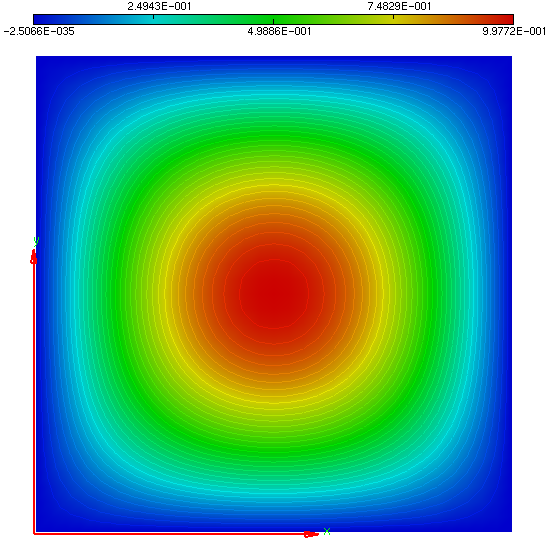
\includegraphics[width=4cm]{direct}
\end{figure}
Different cases of mesh size and time step length were studied to show the dependent of error on the mesh smoothness. We also use two different schemes
\begin{itemize}
	\item Backward Euler scheme
	\begin{figure}[h!]
		\centering
		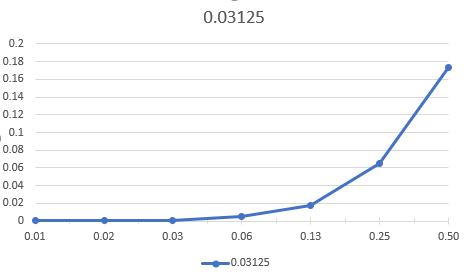
\includegraphics[width=4cm]{graph}
	\end{figure}
	\item Crank-Nicolson scheme
\end{itemize}
The approximate solution at final time is illustrated below.
\subsection{A problem of thermal engineering}
In the aspect of thermal engineering, the simulations of heat transfer attend in several applications. In [...] the author mentioned a realistic heat problem which can be solve by simulating the heat transfer process.\\
Assuming there are two types of material with different thermal conductivity and price. We would like to build a thermal resistance wall from composite plate of the two materials that provide optimal thermal resistance properties and satisfies economical conditions. Let $V$ is the total volume of the plate, $V_e$ and $V_c$ are the volume of expensive and cheap material respectively, then the ratio
$$
\mu = \dfrac{V_e}{V} = \dfrac{V_e}{V_c + V_e}
$$
is fixed. Consider a rectangular room $\Omega_r$ has the size $L_x \times L_y$. At the center of the left wall located a radiator that keep the local temperature at $T_r$, denote as $\Gamma_r$, otherwise as $\Gamma_\alpha$. The thermal flux through the walls is expected to be zero, equivalent to the Neumann boundary condition
$$
\dfrac{\partial u}{\partial n} = 0 \quad \text{on} \quad \Gamma_\alpha.
$$
The right corner of the room is where we place our composite thermal resistance plate. Let $\l_x$ is the width of the plate. The right wall is consider the heat source and gain the Dirichlet boundary condition
$$
u = u_{ext} \quad \text{on} \quad \Gamma_{ext}.
$$
Finally, let $\kappa_a, \kappa_c$ and $\kappa_e$ is correspondingly the thermal conductivity coefficient of air, our cheap and expensive material. Based on our goal of minimizing the temperature inside the room, the cost function can be formulated as follow
$$
J = \dfrac{1}{|\Omega_a|}\int_{0}^{T} \int_{\Omega_a} u dx 
$$
This problem belong to the set of shape optimization problems or more generally is an inverse heat problem. These kinds of problems take part in large amount of engineering applications. An approach is to solve as much acceptable input cases as possible then determine which one is the optimal solution. This way requires numerous computations.
\subsection{Numerical experiment of inverse heat problem}
FreeFem++ provide an efficient tool to handle inverse problems for partial differential equations by using the C++ optimization module IPOPT. To be more accurate, the module support multiple languages in solving optimization problems. The application of IPOPT for solving inverse heat problem is shown below.\\
To use the IPOPT module we have to add command\\
load "ipopt"\\
We need to find the expression of objective function $J$ and its gradient $\nabla J$ respective with the input control function $f$. The optimal $f$ is achieved via IPOPT loop using a conjugate gradient method solver such as Newton-Raphson method.\\
J and gradJ\\
This is an illustrating of the expected control $f$ and its approximation using IPOPT. 

